\documentclass[serif,xcolor=pdftex,dvipsnames,table,hyperref={bookmarks=false}]{beamer}

%%%%%%%%%%%%%%%%
% Change the macros below to configure the title slides
% for your course.
\newcommand{\coursename}{COMPSCI 589}
\newcommand{\instructor}{Benjamin M. Marlin}
\newcommand{\university}{University of Massachusetts Amherst}
\newcommand{\department}{College of Information and Computer Sciences}
%%%%%%%%%%%%%%%%


\newcommand{\settitlecard}[2]{
  \title[\coursename  Lecture #1] 
    {\coursename \\ Lecture #1: #2}
     \author[\instructor]{\instructor}
     \institute[\university]{
     \department\\
     \university
   }
\date{}
}

\newcommand{\maketitlepage}{
  \begin{frame}
  \titlepage
  \center{
    %If you use the slides unmodified, retain the attribution below
    \tiny{Slides by Benjamin M. Marlin (marlin@cs.umass.edu). \\
    \vspace{-1em}Created with support from National Science Foundation Award\# IIS-1350522. 
    %If you modify the slides, please retain the alternate attribution below
    %\tiny{Based on slides by Benjamin M. Marlin (marlin@cs.umass.edu). \\    
    %\vspace{-1em}Created with support from National Science Foundation Award\# IIS-1350522. 
    }                                              
  }  
  \end{frame}
}

\AtBeginSection[]
{
  \begin{frame}<beamer>{Outline}
    \tableofcontents[currentsection,subsectionstyle=hide]
  \end{frame}
}


\newcommand{\cut}[1]{}

\newcommand{\iconbox}[4]{
  \only<#1-#2>{
    \begin{columns}[T]
      \column{0.5in}
           \includegraphics[width=0.5in]{#3}
       \column{3.7in}
            #4
    \end{columns}
    \medskip
    \medskip
    \medskip
  }
}

\mode<presentation>{
  \usepackage{../beamertheme589theme}
  \setbeamercovered{invisible}
}

\mode<handout>{
  \usepackage{../beamertheme589theme}
  \setbeamercovered{transparent}
}


\usepackage[english]{babel}
\usepackage[latin1]{inputenc}
\usepackage{times}
\usepackage[T1]{fontenc}
\usepackage{amsmath}
\usepackage{amssymb}
\usepackage[noend]{algorithmic}
\usepackage{algorithm}
\usepackage{listings}

\renewcommand\mathfamilydefault{\rmdefault}

\newcommand{\setA}{\mathcal{A}}
\newcommand{\setB}{\mathcal{B}}
\newcommand{\setS}{\mathcal{S}}
\newcommand{\setV}{\mathcal{V}}
\DeclareMathOperator*{\union}{\bigcup}
\DeclareMathOperator*{\intersection}{\bigcap}
\DeclareMathOperator*{\Val}{Val}
\newcommand{\mbf}[1]{{\mathbf{#1}}}
\DeclareMathOperator*{\argmax}{arg\,max}
\DeclareMathOperator*{\argmin}{arg\,min}
\DeclareMathOperator*{\sign}{sign}
\newcommand{\deriv}[2]{\frac{\partial{#1}}{\partial{#2}}}


\settitlecard{5}{Support Vector Machines, Basis Expansion and Kernels}

\begin{document}

\maketitlepage

\section{Overview}
\subsection{Foo}

\begin{frame}[t]{Overview}

\begin{itemize}
\setlength{\itemsep}{12pt}
\item To date we've seen one example of a discriminative linear classifier.

\pause \item Today we'll introduce a second example, support vector machines.

\pause \item We'll then address the question of how to increase the capacity of 
linear classifiers so they can produce non-linear classification boundaries.

\end{itemize}

\end{frame}


\section{Support Vector Machines}
\subsection{Foo}

\begin{frame}[t]{Support Vector Machines}

\begin{itemize}
\setlength{\itemsep}{8pt}
\item A binary support vector machine is a discriminative classifier that takes labels in the set $\{-1,1\}$.

\pause\item The decision function has the form:
$$f_{SVM}(\mbf{x}) = \sign(\mbf{w}^T\mbf{x}+b )$$

\pause\item It's easy to show that the decision boundary for logistic regression can be written in exactly the same way.

\pause\item \textbf{Question:} If logistic regression and SVMs have the same form for their decision boundaries, how do the differ?

\end{itemize}
\end{frame}

\begin{frame}[t]{Logistic Loss}

\begin{itemize}
\setlength{\itemsep}{8pt}
\item In the case of logistic regression with $\ell_2$ regularization, we select the model parameters by maximizing the function:

$$C\sum_{i=1}^n \log P(Y=y_i|\mbf{X}=\mbf{x}_i) - ||\mbf{w}||_2^2 $$

\pause\item Under the assumption that the labels take the values $\{-1,1\}$, it can be shown that
this is equivalent to minimizing the function:

$$C\sum_{i=1}^n \log(1+\exp(-y_i \cdot g(\mbf{x}))) + ||\mbf{w}||_2^2$$

where $L_{log}(y_i,g(\mbf{x}_i)) = \log(1+\exp(-y_i \cdot g(\mbf{x})))$ is the \textit{logistic loss function} and 
$g(\mbf{x}) = \mbf{w}^T\mbf{x}+b$.


\end{itemize}
\end{frame}

\begin{frame}[t]{Hinge Loss}

\begin{itemize}
\setlength{\itemsep}{8pt}
\item In the case of SVMs with $\ell_2$ regularization, we select the model parameters by minimizing the function:

\begin{align*}
C\sum_{i=1}^n \max(0,1-y_i \cdot g(\mbf{x}_i)) +  ||\mbf{w}||_2^2 
\end{align*}

\pause\item The function $L_{h}(y_i,g(\mbf{x}_i))= \max(0,1-y_i \cdot g(\mbf{x}_i))$ is called the \textit{hinge loss}.

\end{itemize}
\end{frame}

\begin{frame}[t]{Zero-One Loss}

\begin{itemize}
\setlength{\itemsep}{8pt}
\item Both the logistic loss and the hinge loss are convex upper bounds on the zero-one loss:

$$L_{01}(y_i,g(\mbf{x}_i)) = \mathbb{I}[y_i \neq \sign(g(\mbf{x}_i))]$$

\pause\item The average zero-one loss over a data set is exactly the classification error rate.

\pause\item This is the loss function we'd like to minimize, but this generally isn't computationally feasible, thus the need for surrogate loss functions.

\pause\item Hinge loss has some advantages over logistic loss, as we'll see.


\end{itemize}
\end{frame}


\begin{frame}[t]{Maximum Margin Property}

Part of popularity of SVMs stems from the fact that the hinge loss results in the \textit{maximum margin} decision boundary when the training cases are linearly separable.

\center
\begin{minipage}{2in}
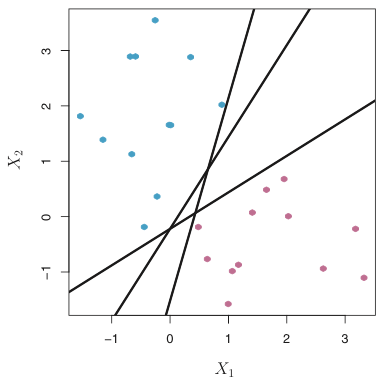
\includegraphics[width=2in]{../Figures/svm-boundaries.png}
\end{minipage}%
\begin{minipage}{2in}
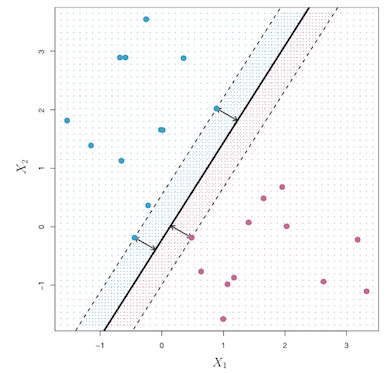
\includegraphics[width=2in]{../Figures/svm-opt.png}
\end{minipage}

\end{frame}

\begin{frame}[t]{Support Vector Property}

In the linearly separable case, some data points will always fall exactly on the margins. These points are called \textit{support vectors}.

\center
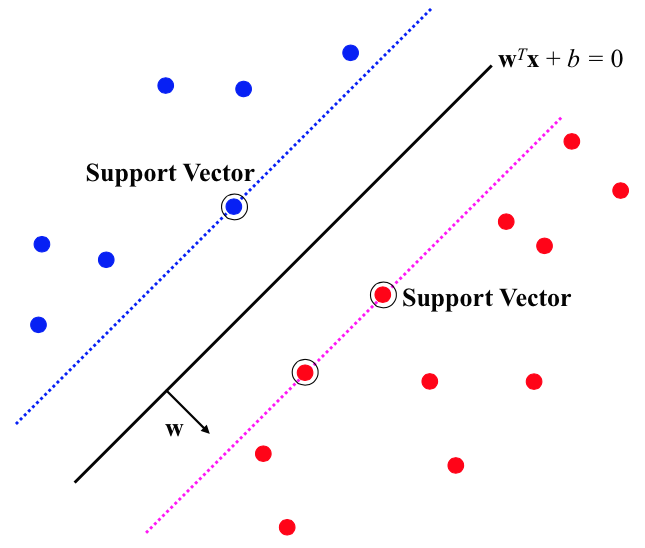
\includegraphics[width=2.5in]{../Figures/svm-support-vectors.png}

\end{frame}

\begin{frame}[t]{SVMs vs Logistic Regression}

\begin{itemize}
\setlength{\itemsep}{8pt}
\item SVMs and Logistic regression are both discriminative linear classifiers with identical capacity and space complexity. 

\pause\item SVMs and Logistic regression have very similar convex loss functions and identical regularizers.

\pause\item The hinge loss is not differentiale, unlike the logistic loss, so SVMs require more advanced optimization methods (sub-gradient descent or quadratic programming), but there are extremely good algorithms and implementations available.

\pause \item The maximum-margin property of SVMs can yield better generalization than logistic regression when data is scarce.

\end{itemize}
\end{frame}

\begin{frame}[t]{SVMs vs Logistic Regression}

\begin{itemize}
\setlength{\itemsep}{8pt}

\item It is somewhat more difficult to form a multi-class SVM than a multi-class logistic regression model, and many implementations use ``hacks'' like one-vs-all.

\pause \item Unlike logistic regression, SVMs do not produce probabilistic outputs, but again, there are hacks that can estimate probabilities.

\end{itemize}
\end{frame}

\section{Basis Expansion and Kernels}
\subsection{Foo}


\begin{frame}[t]{The Problem with Linear Models}

\begin{itemize}
\setlength{\itemsep}{8pt}
\item The problem with linear classifiers is that their decision boundaries are by definition linear in the input feature space.

\pause\item This means that they can have very high bias on complex data.

\pause\item \textbf{Question:} How can we relax the constraint of linear decision boundaries while retaining the nice properties of linear classifiers?

\end{itemize}
\end{frame}

\begin{frame}[t]{Basis Function Expansion}

\begin{itemize}
\setlength{\itemsep}{8pt}
\item One very simple solution is to apply a set of functions $\phi_1$,...,$\phi_K$ to the
raw feature vector $\mbf{x}$ to map it in to a new feature space:

$$\phi(\mbf{x}) = [\phi_1(\mbf{x}),...,\phi_K(\mbf{x})]$$

\pause \item This is called a \textit{basis function expansion} since $K>D$ in general. This requires that we know the functions $\phi_1$,...,$\phi_K$ that we want to apply in advance.

\pause\item We then define a linear classifier (SVM or Logistic Regression) in this new feature space:

$$\mbf{w}^T\phi(\mbf{x}) + b$$

\end{itemize}
\end{frame}

\begin{frame}[t]{Basis Function Expansion Examples}

\begin{itemize}
\setlength{\itemsep}{8pt}
\item \textbf{Degree 2 Polynomial Basis:} We include all single features $x_d$, their squares $x_d^2$, and all products of two distinct features $x_dx_{d'}$.

\pause \item \textbf{Degree $B$ Polynomial Basis:} We include all single features $x_d$, and all unique products of between $2$ and $B$ features.

\pause \item The problem is that the space complexity of representing the expanded set of features is essentially $O(D^B)$.

\pause \item Next we'll see how this problem can be solved.

\end{itemize}
\end{frame}

\section{Kernels}
\subsection{foo}

\begin{frame}[t]{Representer Theorem}

\begin{itemize}
\setlength{\itemsep}{8pt}
\item One of the interesting properties of SVMs is that the optimal weight vectors can always be expressed as a weighted linear combination of the data vectors:

$$\mbf{w} = \sum_{j=1}^N \alpha_j \mbf{x}_j$$

\pause\item This result is called the \textit{representer theorem}. 

\end{itemize}
\end{frame}

\begin{frame}[t]{Dependence on Inner Products}

\begin{itemize}
\setlength{\itemsep}{8pt}
\item Plugging this result back in to the SVM objective we find that the objective only depends on the data through inner products: $\mbf{x}_j^T\mbf{x}_i$:

\begin{align*}
g(\mbf{x}_i) &= \mbf{w}^T\mbf{x}_i + b 
= \sum_{j=1}^N \alpha_j \mbf{x}_j^T\mbf{x}_i +b\\
||\mbf{w}||_2^2 &= \mbf{w}^T\mbf{w} 
= \sum_{j=1}^N \sum_{i=1}^N \alpha_j\alpha_i \mbf{x}_j^T\mbf{x}_i
\end{align*}


\end{itemize}
\end{frame}

\begin{frame}[t]{Basis Expansion and Representer Theorem}

\begin{itemize}
\setlength{\itemsep}{8pt}
\item Under an arbitrary basis expansion $\phi(\mbf{x})$ this result becomes:

\begin{align*}
g(\phi(\mbf{x}_i)) &= \sum_{j=1}^N \alpha_j \phi(\mbf{x}_j)^T\phi(\mbf{x}_i) +b\\
||\mbf{w}||_2^2  &= \sum_{j=1}^N \sum_{i=1}^N \alpha_j\alpha_i \phi(\mbf{x}_j)^T\phi(\mbf{x}_i) \\
\end{align*}

\item It can be shown in the linearly separable case that the $\alpha_i$ parameters
for data cases that are not support vectors are always $0$.

\end{itemize}
\end{frame}

\begin{frame}[t]{The Kernel Trick}

\begin{itemize}
\setlength{\itemsep}{8pt}
\item Amazingly, for many useful basis function expansions $\phi(\mbf{x})$, it is possible to find a function $\mathcal{K}(\mbf{x},\mbf{x}') =\phi(\mbf{x})^T\phi(\mbf{x}')$ that can compute the inner product under the basis expansion \textbf{without ever explicitly performing the basis function expansion}!

\pause \item Such functions are called \textit{kernel functions} and this is known as the ``Kernel Trick''.

\pause \item Importantly, you can also directly learn the parameters $\alpha_i$ and $b$ using the kernel trick, without constructing the basis expansion.

\pause\item Interestingly, there exist kernels for which the basis function expansion implied by the kernel isn't even finite dimensional!


\end{itemize}
\end{frame}

\begin{frame}[t]{Examples of Kernel Functions}

\begin{itemize}
\setlength{\itemsep}{8pt}
\item \textbf{Degree $B$ Polynomial Kernel:} $\mathcal{K}_P(\mbf{x},\mbf{x}') = (\mbf{x}^T\mbf{x}' + 1)^B$

\pause \item \textbf{Gaussian/RBF Kernel:} $\mathcal{K}_G(\mbf{x},\mbf{x}') = \exp(-\gamma||\mbf{x}-\mbf{x}'||_2^2)$

\pause \item Many more domain-specific kernels for strings, histograms, probability distributions, and other complex structured objects.

\end{itemize}
\end{frame}


\begin{frame}[t]{Trade-Offs: Basis Expansion and Kernels}

\begin{itemize}
\setlength{\itemsep}{8pt}
\item Linear classifiers are fast and space efficient, but can have high bias.

\pause \item Basis expansion requires more space ($O(NK)$ for data and $O(K)$ for parameters), but yields non-linear classifiers that have lower bias.

\pause \item Kernel SVMs actually require $O(N^2)$ space for storing all the kernel values during training and have $O(N)$ parameters. This can still be much lower than $O(NK)$ for large sets of basis functions. Kernels also yield non-linear classifiers that have lower bias.

\pause\item Kernel SVMs often have at least two parameters ($C$ and a kernel hyperparameter). These need to be set jointly, which can be computationally expensive. 

\end{itemize}
\end{frame}

\begin{frame}[t]{Trade-Offs: Basis Expansion and Kernels}

\begin{itemize}
\setlength{\itemsep}{8pt}

\item Gaussian kernel SVMs also have infinite capacity, and a very closely related to weighted KNN.

\pause\item Importantly, everything we said about SVMs and kernels is also true for logistic regression. Applying the kernel trick to logistic regression yields a model called ``kernel logistic regression'' or KLR.

\pause\item KLR can exploit infinite dimensional feature spaces, can be learned with smooth optimization methods, supports probabilistic outputs, and has an easy multi-class generalization, but lacks the margin maximization property. 

\end{itemize}
\end{frame}


\end{document}
